\documentclass{beamer}
\usetheme{Madrid}

\usepackage[utf8]{inputenc}
\usepackage{graphicx}

\title[Michelson Interferometry]{Wavelength Detection through Michelson Interferometry}
\author{Henry Shackleton}

\begin{document}

\titlepage

\begin{frame}
  \frametitle{Outline}
\tableofcontents
\end{frame}

\section{Introduction and Theory}


\begin{frame}
  \frametitle{What is Michelson Interferometry?}
  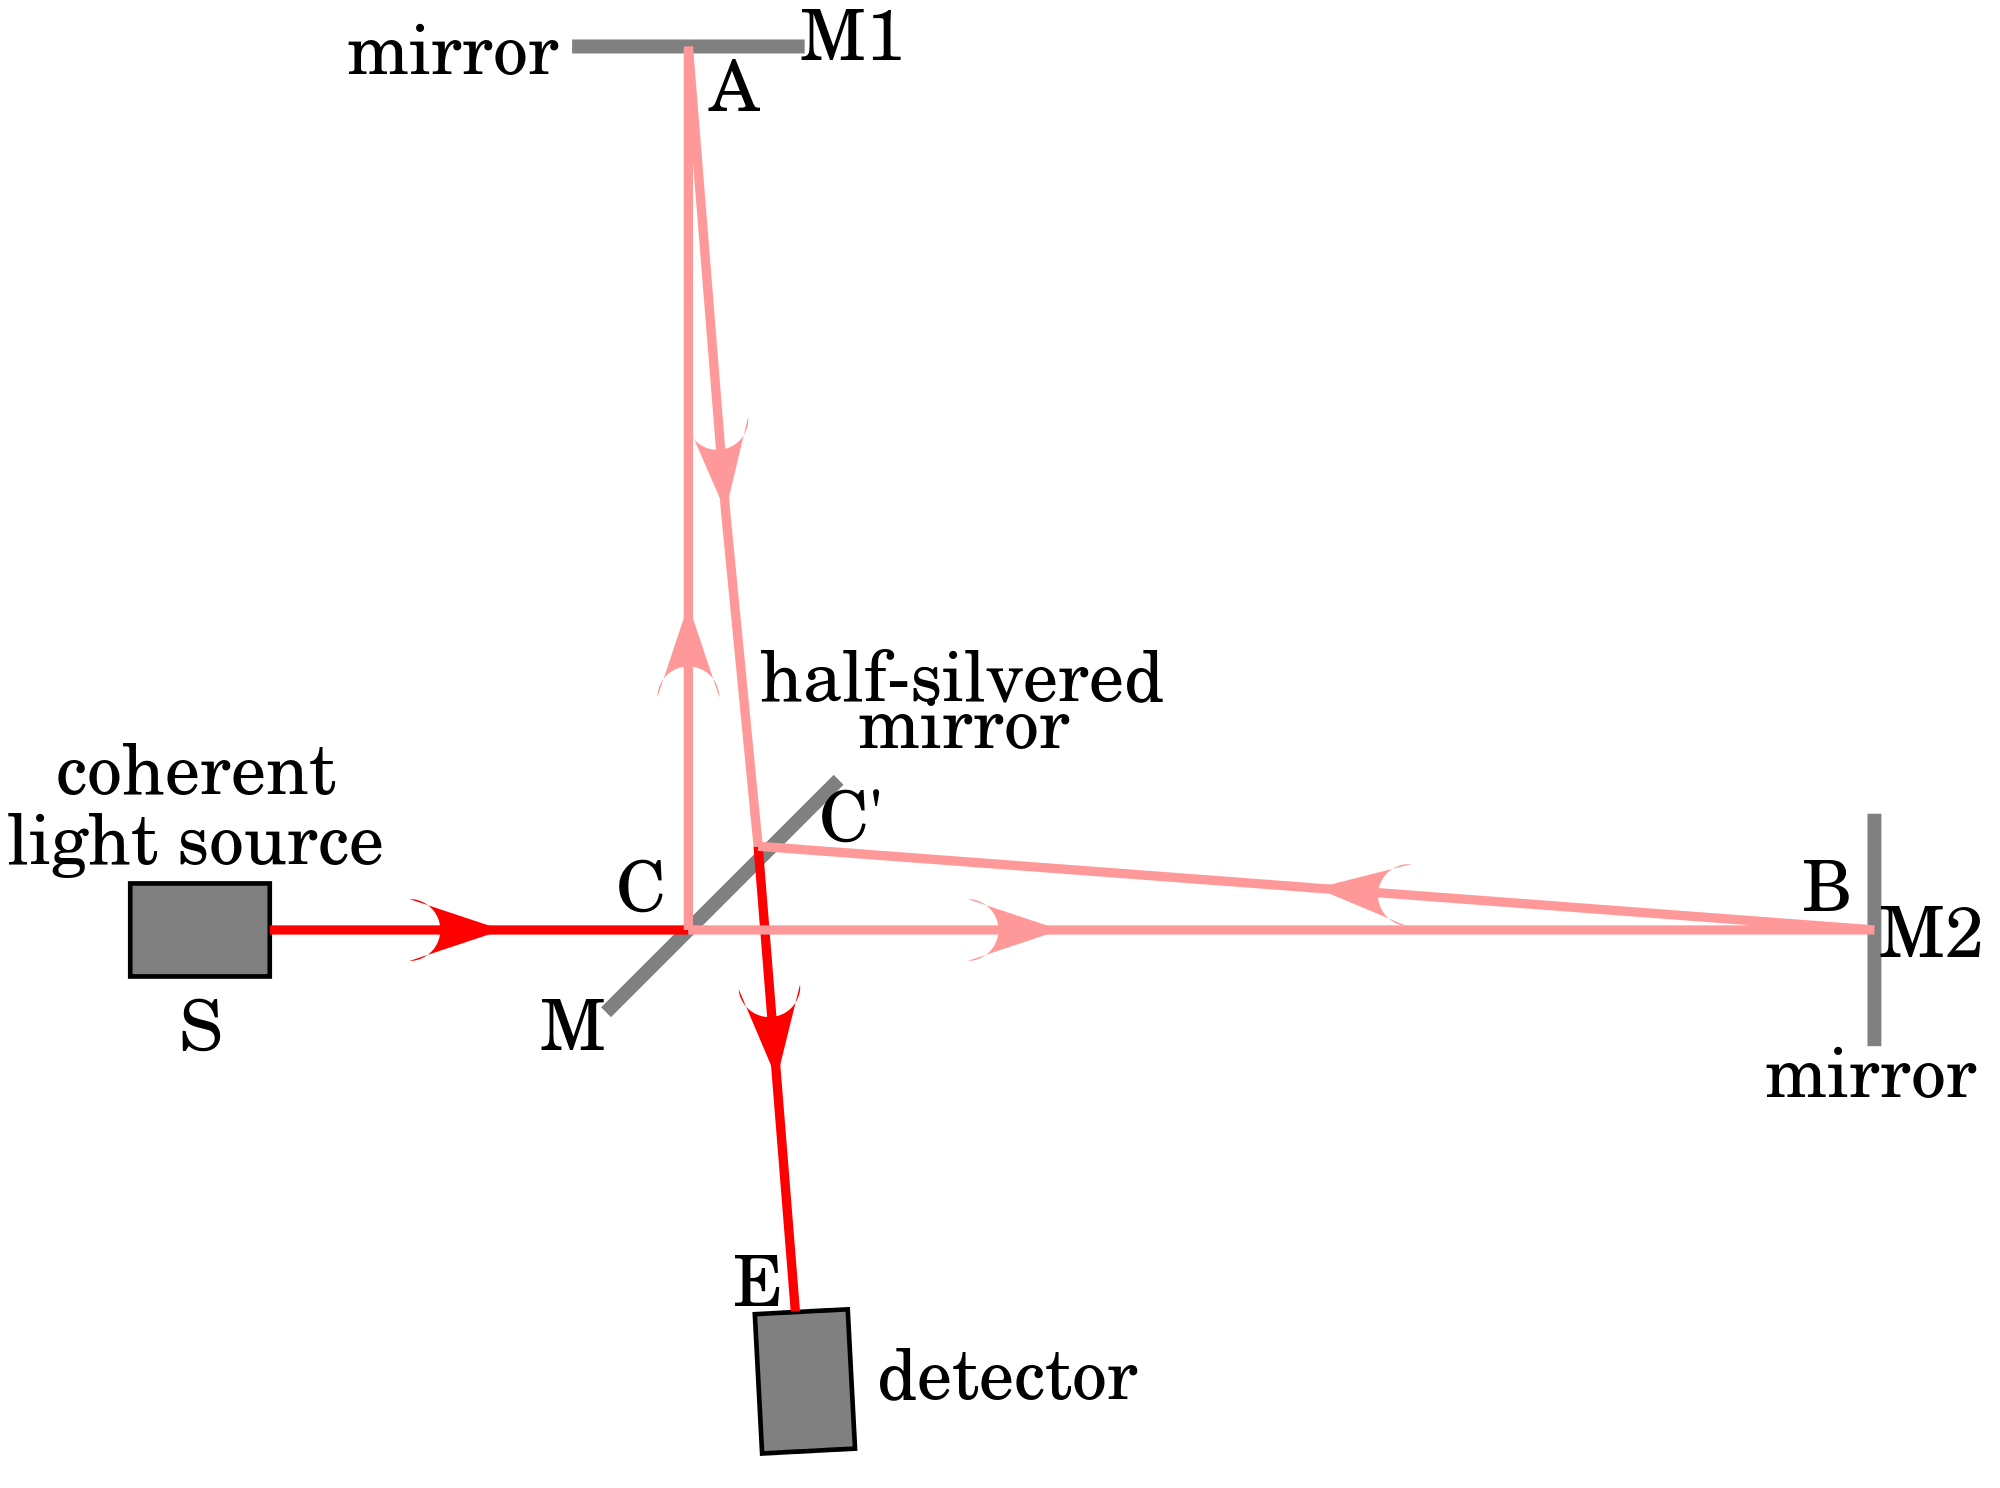
\includegraphics[width=9cm]{basic_interferometer.png}
  \pause

  Use detector measurements to determine wavelength of light source.
\end{frame}

\begin{frame}
  \frametitle{Light travels as waves}
  \begin{equation*}
    E(t) = E_1 e^{i\left(\phi_1 - \omega t\right)}
  \end{equation*}
  \hspace{5pt}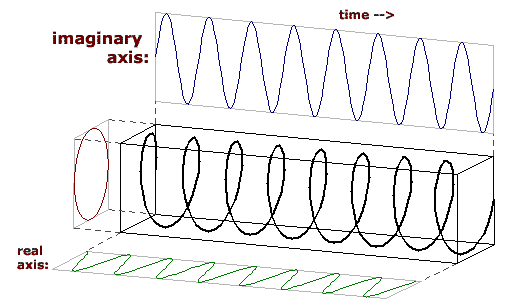
\includegraphics[width=10cm]{complex.png}
\end{frame}

\begin{frame}
  \frametitle{Superposition of waves work as addition}
  \begin{center}
  \begin{equation*}
    E_T(t) = E_1 e^{i(\phi_1 - \omega t)} + E_2 e^{i(\phi_2 - \omega t)}
  \end{equation*}
\end{center}
\end{frame}

\begin{frame}
  \frametitle{From complex waves to observables}
  \begin{itemize}
    \item
    What photodetectors observe is the \textit{intensity} of a wave.
  \item
    $I \propto \langle E_T^* E_T \rangle = E_1^2 + E_2^2 + 2 E_1 E_2 \cos(\phi_1 - \phi_2)$
  \item Relative phase difference affects intensity measured.
    \pause
    \begin{itemize}
      \item $\phi_1 - \phi_2 = 2 \pi n$, $n = 1, 2, \ldots$ - constructive interference
        \pause
      \item $\phi_1 - \phi_2 = (2n + 1) \pi$ - destructive interference
    \end{itemize}
\end{itemize}
\end{frame}

\begin{frame}
  \frametitle{Relative length traveled to relative phase}
  \begin{itemize}
    \item One wave travels a length $2l_1$, and one wave travels a length $2l_2$. What is the relative phase offset of the two?
    \end{itemize}
  \begin{equation*}
    \phi_1 - \phi_2 = \frac{4\pi}{\lambda} \left(l_2 - l_1 \right)
  \end{equation*}
  \pause
    \begin{equation*} 
      I \propto E^2  + E^2 \cos\left(\frac{4\pi}{\lambda} (l_2 - l_1) \right)
    \end{equation*}
  \end{frame}

\section{Experimental Setup}
\begin{frame}
  \frametitle{Overview of experimental setup}
  \hspace{25pt}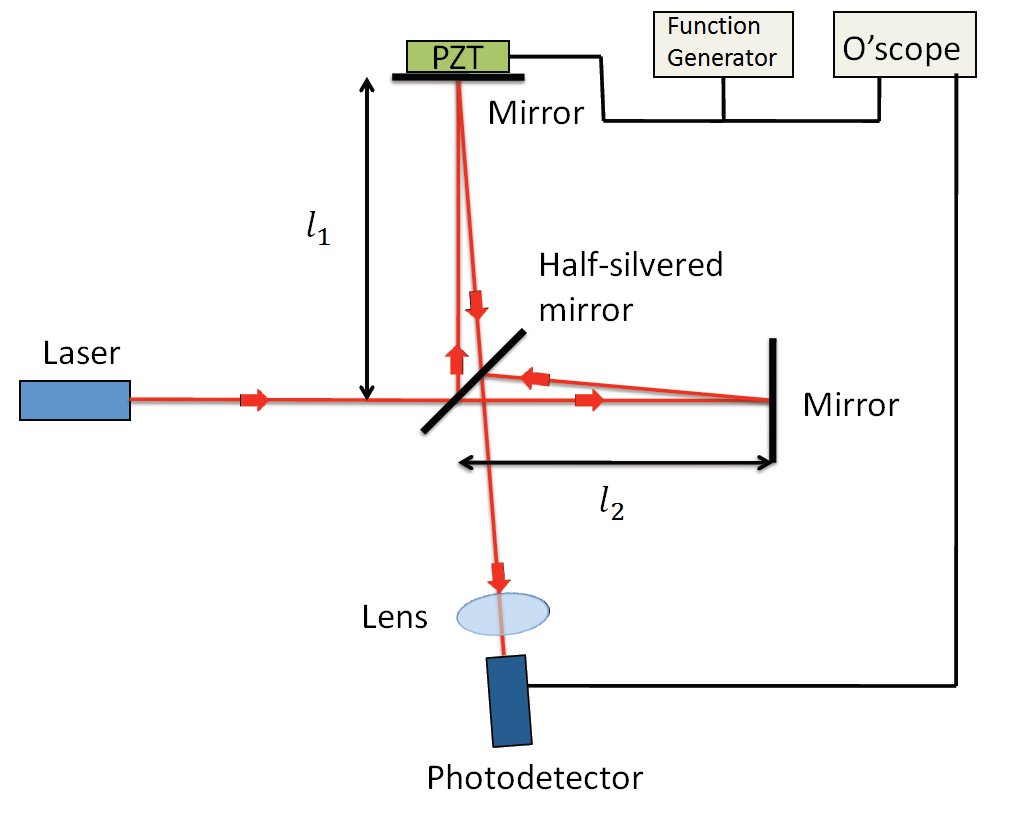
\includegraphics[width=10cm]{setup.png}
\end{frame}

\begin{frame}
  \frametitle{PZT converts voltage to displacement}
  \begin{itemize}
    \item PZT changes relative length difference from $2(l_2 - l_1)$ to $2(l_2 - l_1 - \Delta V)$.
    \item Linear relative length difference causes a linear phase difference proportional to the wavelength.
    \item Linear phase difference causes periodic intensity differences.
    \item Measure voltage differences corresponding to a full period in intensity.
  \end{itemize}
\end{frame}

\begin{frame}
  \frametitle{Oscilliscope display of interference patterns}
  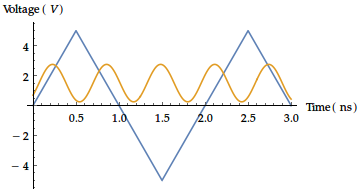
\includegraphics[width=12cm]{waveform}
\end{frame}

\section{Data Analysis}

\begin{frame}
  \frametitle{Distribution of measured voltage differences}
  \begin{columns}
    \begin{column}{0.5\textwidth}
  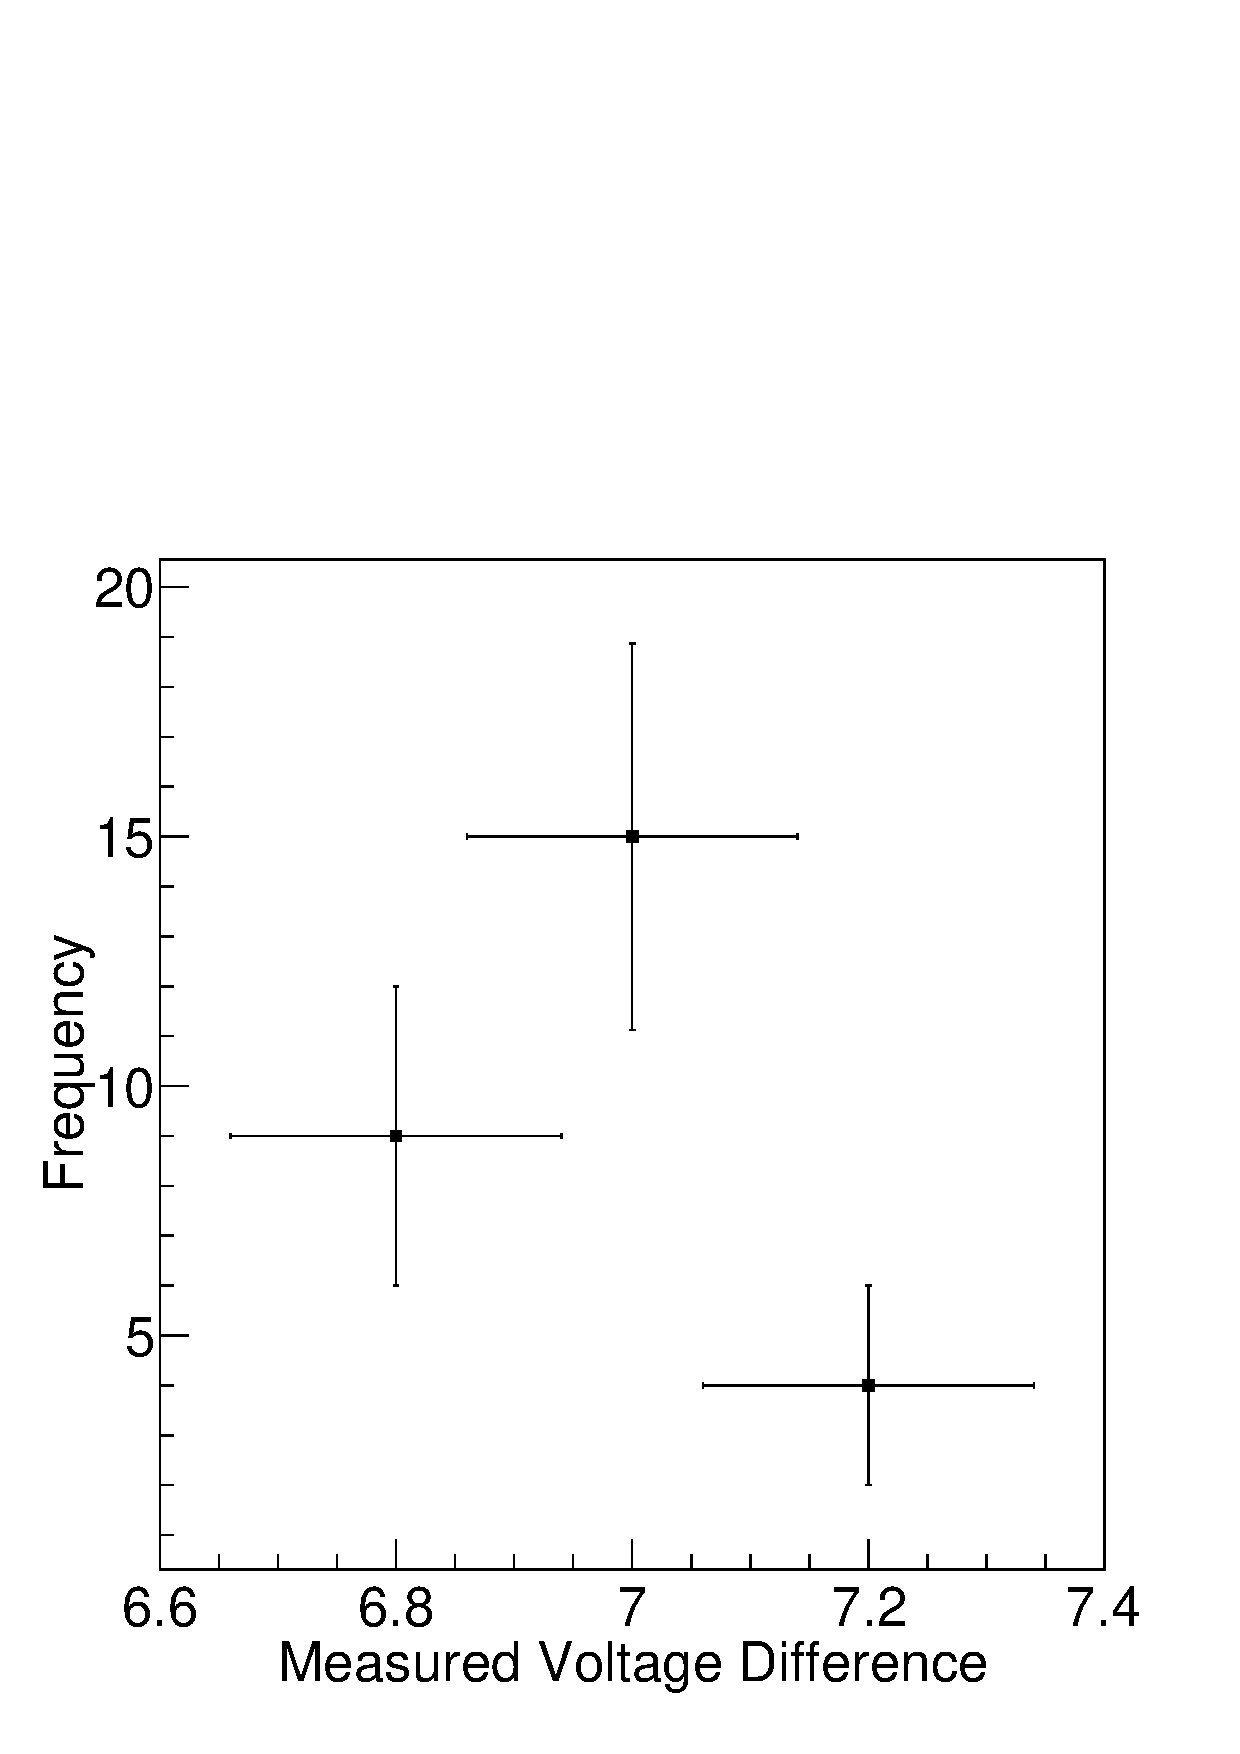
\includegraphics[width=6.5cm]{graph_helvetica}
\end{column}

\begin{column}{0.5\textwidth}
  \begin{itemize}
    \item Individual measured voltage differences give error of $\pm 0.14$ V from measurement
      \pause
    \item Averaging voltage differences gives $6.96 \pm .02$ V 
      \pause
    \item Total uncertainty in voltage $6.96 \pm .14$ V
      \pause
    \item PZT voltage to length conversion $44.6 \pm 2.6$ nm/V
      \pause
    \item $\lambda = 620 \pm 38$ nm
  \end{itemize}
  \end{column}
\end{columns}
\end{frame}

\begin{frame}
  \frametitle{Predicted wavelength agrees with independent calculations}
  \begin{itemize}
    \item Wavelength reported on laser is 594.6 nm.
  \item Predicted wavelength of $620 \pm 38$ nm mostly falls within this range.
  \item Michelson interferometry can be used to accurately calculate wavelengths.
\end{itemize}
\end{frame}

\section{Conclusion}

\begin{frame}
  \frametitle{Wavelength calculation through Michelson interferometry}
  \begin{itemize}
    \item Michelson interferometers produce interference patterns dependent on the light wavelength and the relative length difference between the two arms.
      \pause
    \item By controlling this length with a PZT, we can accurately determine the wavelength of the light source.
      \pause
    \item Error propegation is largely controlled by the PZT.
      \pause
    \item The aether probably doesn't exist.
  \end{itemize}
\end{frame}

\begin{frame}
  \frametitle{Derivation of wavelength/voltage correpondance}
  \begin{center}
  \begin{equation*}
    I \propto E^2\left(1 + cos\left(\frac{4\pi}{\lambda} (l_2 - l_1 - \Delta V ) \right) \right)
  \end{equation*}
  One period with respect to $V$ given by
  \begin{equation*}
    2 \pi V = \frac{4 \pi \Delta}{\lambda}
    \\
    \lambda = \frac{2 \Delta}{V}
  \end{equation*}
\end{center}
\end{frame}

\begin{frame}
  \frametitle{Constructive interference in light waves}
  \begin{center}
    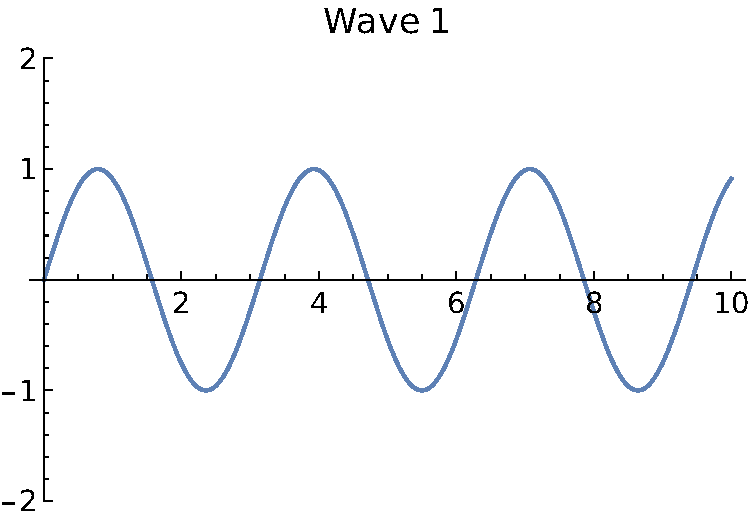
\includegraphics[width=5cm]{wave1pres}
    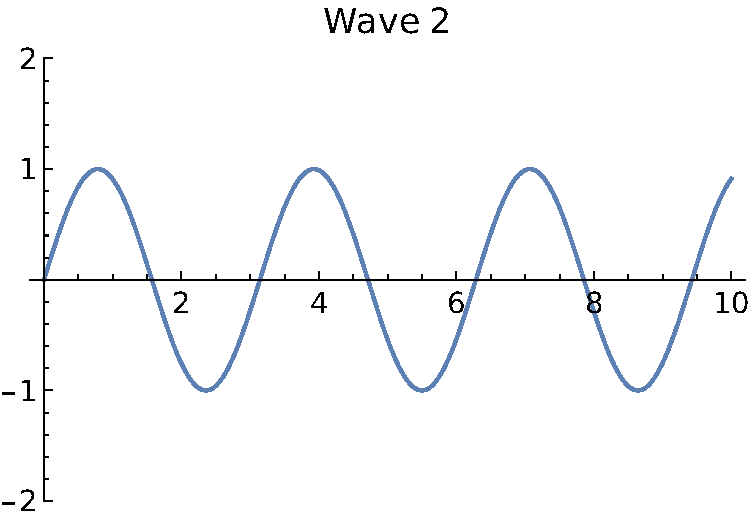
\includegraphics[width=5cm]{wave2pres}
    \\
    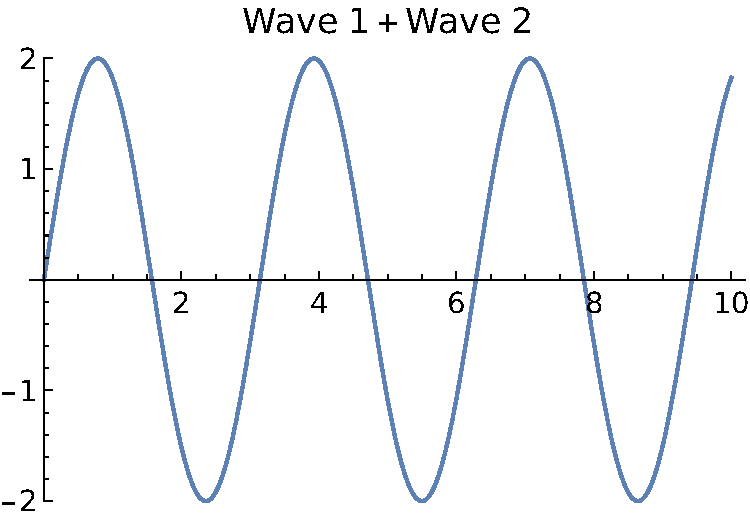
\includegraphics[width=5cm]{constructivepres}
    \end{center}
  \end{frame}

\begin{frame}
  \frametitle{Constructive interference in light waves}
  \begin{center}
    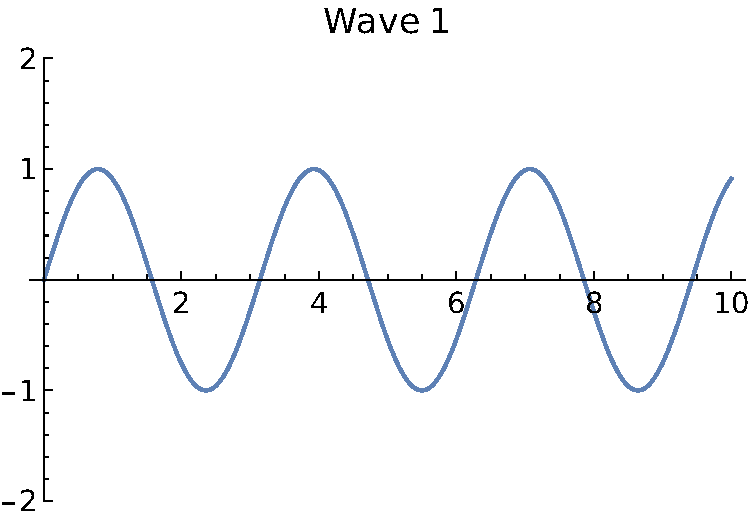
\includegraphics[width=5cm]{wave1pres}
    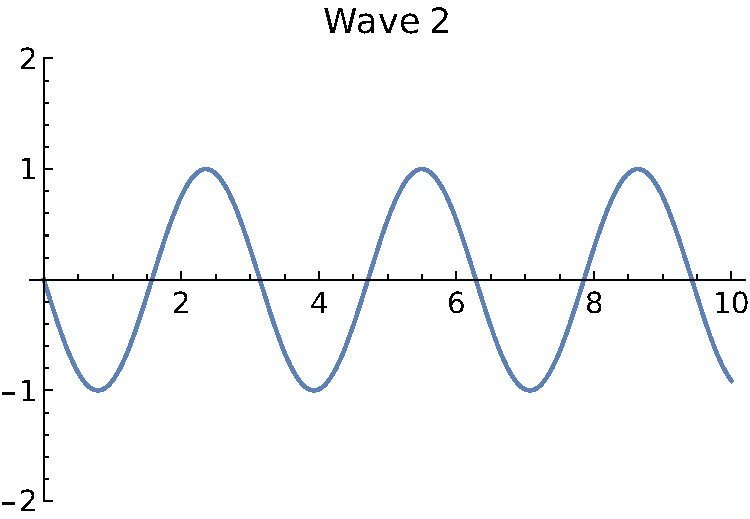
\includegraphics[width=5cm]{wave3pres}
    \\
    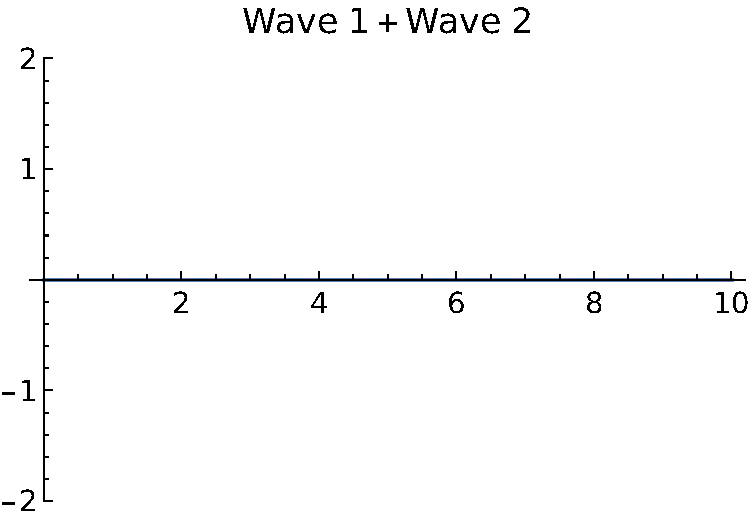
\includegraphics[width=5cm]{destructivepres}
  \end{center}
\end{frame}

\end{document}
